% ------------------------------------------------------------------
\documentclass[12 pt]{article} % A4 paper set by geometry package below
\pagenumbering{arabic}
\setlength{\parindent}{10 mm}
\setlength{\parskip}{12 pt}

% Nimbus Sans font should be reasonably legible
\usepackage{helvet}
\renewcommand{\familydefault}{\sfdefault}
\usepackage[T1]{fontenc}  % Without this \textsterling produces $

% Section header spacing
\usepackage{titlesec}
\titlespacing\section{0pt}{12pt plus 4pt minus 2pt}{0pt plus 2pt minus 2pt}
\titlespacing\subsection{0pt}{12pt plus 4pt minus 2pt}{0pt plus 2pt minus 2pt}
\titlespacing\subsubsection{0pt}{12pt plus 4pt minus 2pt}{0pt plus 2pt minus 2pt}

\usepackage{amsmath}
\usepackage{amssymb}
\usepackage{graphicx}
\usepackage{verbatim}    % For comment
\usepackage[shortlabels]{enumitem}
\usepackage[paper=a4paper, marginparwidth=0 cm, marginparsep=0 cm, top=2.5 cm, bottom=2.5 cm, left=3 cm, right=3 cm, includemp]{geometry}
\usepackage[pdftex, pdfstartview={FitH}, pdfnewwindow=true, colorlinks=true, citecolor=blue, filecolor=blue, linkcolor=blue, urlcolor=blue, pdfpagemode=UseNone]{hyperref}

% Put module code and last-modified date in footer
\usepackage{fancyhdr}
\pagestyle{fancy}
\fancyhf{}
\renewcommand{\headrulewidth}{0pt}
\cfoot{{\small \thisweek}\hfill \thepage\hfill {\small \moddate}}

% Hopefully address Canvas complaints about pdf tagging
%\usepackage[tagged]{accessibility}
% ------------------------------------------------------------------



% ------------------------------------------------------------------
% Shortcuts
\newcommand{\la}{\ensuremath{\lambda} }
% ------------------------------------------------------------------



% ------------------------------------------------------------------
\begin{document}
\newcommand{\thisweek}{MATH327 Extra (Dalton)}
\newcommand{\moddate}{Last modified 21 May 2021}
\begin{center}
  {\Large \textbf{MATH327: Statistical Physics, Spring 2021}} \\[12 pt]
  {\Large \textbf{Extra practice \ --- \ Dalton's law}} \\[24 pt]
\end{center}

Consider the mixture of two ideal gases analyzed in Question~1 of the second homework assignment.
As illustrated below, the two gases with particle numbers $N_1$ and $N_2$ are in a container of volume $V$ at temperature $T$.
Within each gas the particles are indistinguishable, but particles of one gas are distinguishable from particles of the other gas.
Their thermal de~Broglie wavelengths and single-particle canonical partition functions are
\begin{align*}
  \la_i(T) & = \sqrt{\frac{2\pi\hbar^2}{m_i T}} &
  Z_1^{(i)}(T) & = \frac{V}{\la_i^3},
\end{align*}
where $m_1$ and $m_2$ are the masses of particles in the two different gases.

\begin{center}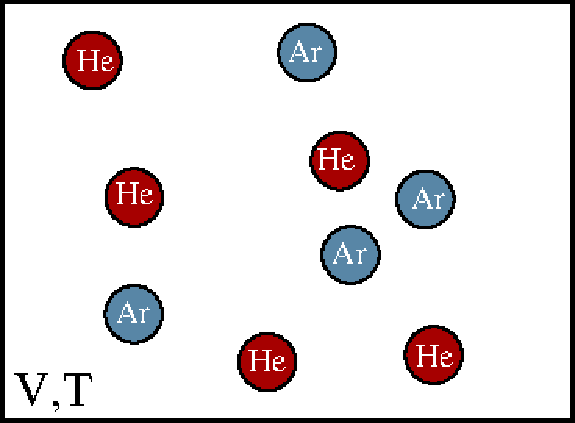
\includegraphics[width=0.5\textwidth]{figs/mixed.pdf}\end{center}

Determine the equation of state for the mixture, and use it to demonstrate Dalton's law,
\begin{equation*}
  P = P_1 + P_2,
\end{equation*}
where the `partial pressures' obey
\begin{align*}
  P_1 V & = N_1 T &
  P_2 V & = N_2 T.
\end{align*}

\end{document}
% ------------------------------------------------------------------
